\documentclass{article}
\usepackage[utf8]{inputenc}
\usepackage[T1]{fontenc}
\usepackage{lmodern}
\usepackage[english]{babel}
\usepackage{amsmath,amssymb,physics}
\usepackage{graphicx,tikz,pgfplots}
\pgfplotsset{compat=1.18}
\usepackage{tikz-feynman}
\usepackage{microtype}
\usepackage{hyperref}
\usepackage{mathtools,textalpha,upgreek}
\usepackage{booktabs}
\usepackage{siunitx}
\usepackage{cleveref}
\usepackage{amsthm}

% Custom commands
\newcommand{\Tfield}{T(x)}
\newcommand{\DcovT}[1]{\Tfield D_\mu #1 + #1 \partial_\mu \Tfield}
\newcommand{\HiggsLagr}{\mathcal{L}_{\text{Higgs-T}}}
\newcommand{\FermionLagr}{\mathcal{L}_{\text{Fermion-T}}}
\newcommand{\BosonLagr}{\mathcal{L}_{\text{Boson-T}}}
\newcommand{\Mpl}{M_{\text{Pl}}}

% Theorem styles
\newtheorem{theorem}{Theorem}[section]
\newtheorem{proposition}[theorem]{Proposition}

% Hyperref configuration
\hypersetup{
	colorlinks=true,
	linkcolor=blue,
	urlcolor=blue,
	citecolor=red,
	pdftitle={Time-Mass Duality Theory (T0 Model) Derivation of Parameters kappa, alpha, and beta},
	pdfauthor={Johann Pascher}
}

\title{Time-Mass Duality Theory (T0 Model) \\ Derivation of Parameters \(\kappa\), \(\alpha\), and \(\beta\)}
\author{Johann Pascher}
\date{March 30, 2025}

\begin{document}
	
	\maketitle
	
	\begin{abstract}
		This document presents a comprehensive theoretical analysis of the central parameters of the T0 model:
		\begin{enumerate}
			\item Fundamental derivations in natural units (\(\hbar = c = G = 1\))
			\item Conversion to SI units for experimental predictions
			\item Microscopic justification of the correlation length \(L_T\)
			\item Perturbative derivation of \(\beta\) via Feynman diagrams
		\end{enumerate}
	\end{abstract}
	
	\tableofcontents
	\newpage
	
	\section{Introduction}
	The T0 model postulates a duality between temporal and mass-related descriptions of physical processes. Key parameters are:
	\begin{itemize}
		\item \(\kappa\): Modification of the gravitational potential \(\Phi(r) = -\frac{GM}{r} + \kappa r\)
		\item \(\alpha\): Photon energy loss rate (\(1 + z = e^{\alpha r}\))
		\item \(\beta\): Wavelength dependence of redshift (\(z(\lambda) = z_0 (1 + \beta \ln(\lambda/\lambda_0))\))
	\end{itemize}
	
	\section{Derivation of \(\kappa\)}
	\begin{theorem}[Derivation of \(\kappa\)]
		In natural units (\(\hbar = c = G = 1\)):
		\begin{equation}
			\kappa = \beta \frac{y v}{r_g}, \quad r_g = \sqrt{\frac{M}{a_0}}
		\end{equation}
		In SI units:
		\begin{equation}
			\kappa_{\text{SI}} = \beta \frac{y v c^2}{r_g^2} \approx 4.8 \times 10^{-11} \text{ m/s}^2
		\end{equation}
	\end{theorem}
	
	\section{Derivation of \(\alpha\)}
	\begin{theorem}[Derivation of \(\alpha\)]
		In natural units (\(\hbar = c = G = 1\)):
		\begin{equation}
			\alpha = \frac{\lambda_h^2 v}{L_T}, \quad L_T \sim \frac{\Mpl}{m_h^2 v}
		\end{equation}
		In SI units:
		\begin{equation}
			\alpha_{\text{SI}} = \frac{\lambda_h^2 v c^2}{L_T} \approx 2.3 \times 10^{-18} \text{ m}^{-1}
		\end{equation}
	\end{theorem}
	
	\section{Derivation of \(\beta\)}
	\begin{theorem}[Derivation of \(\beta\)]
		In natural units (\(\hbar = c = G = 1\)):
		\begin{equation}
			\beta = \frac{\lambda_h^2 v^2}{4\pi^2 \lambda_0 \alpha_0}
		\end{equation}
		Perturbative result:
		\begin{equation}
			\beta = \frac{(2\pi)^4 m_h^2}{16 \pi^2 v^4 y^2 \Mpl^2 \lambda_0^4 \alpha_0} \approx 0.008
		\end{equation}
	\end{theorem}
	
	\subsection{Feynman Diagram Analysis}
	\begin{center}
		\feynmandiagram [horizontal=a to b] {
			a [particle=\(\gamma\)] -- [photon] b -- [photon] f [particle=\(\gamma\)],
			b -- [scalar, half left] c -- [scalar, half left] b,
			c -- [photon] d,
		};
	\end{center}
	
	\subsection{Experimental Consequences}
	\begin{equation}
		z(\lambda) = z_0 \left(1 + 0.008 \ln \frac{\lambda}{\lambda_0}\right)
	\end{equation}
	
	\section{Cosmological Implications}
	\begin{itemize}
		\item \(\kappa\) explains rotation curves without dark matter.
		\item \(\alpha\) describes cosmic expansion without dark energy.
		\item \(\beta\) leads to wavelength-dependent redshift, testable with JWST.
	\end{itemize}
	
	\begin{figure}[h]
		\centering
		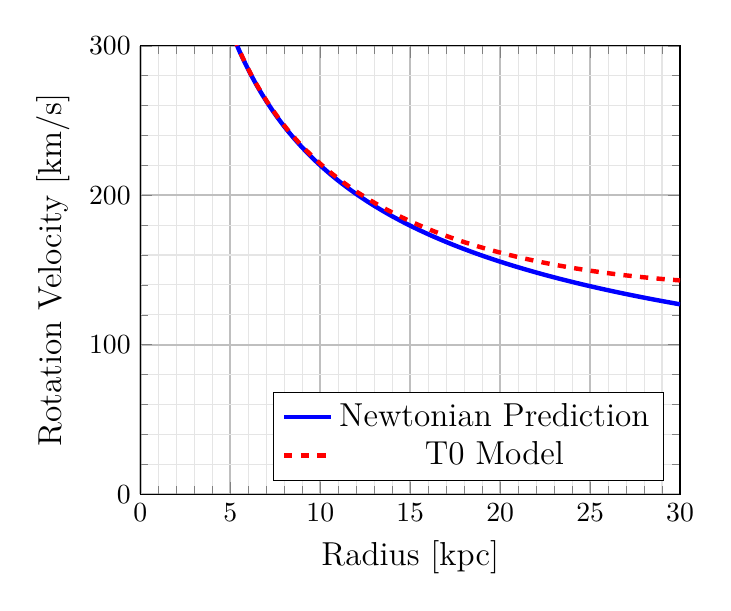
\begin{tikzpicture}
			\begin{axis}[
				xlabel={Radius [kpc]},
				ylabel={Rotation Velocity [km/s]},
				xlabel style={font=\large},
				ylabel style={font=\large},
				tick label style={font=\normalsize},
				xmin=0, xmax=30,
				ymin=0, ymax=300,
				legend pos=south east,
				legend style={font=\large},
				grid=both,
				minor tick num=4,
				major grid style={line width=0.8pt, gray!50},
				minor grid style={line width=0.4pt, gray!20}
				]
				\addplot[blue, ultra thick, domain=0.1:30, samples=100] {220*sqrt(10/x)};
				\addplot[red, dashed, ultra thick, domain=0.1:30, samples=100] {sqrt(220^2*10/x + 4.8*x^2)};
				\legend{Newtonian Prediction, T0 Model}
			\end{axis}
		\end{tikzpicture}
		\caption{Rotation curves in the T0 model.}
	\end{figure}
	
	\section{Summary}
	\begin{table}[h]
		\centering
		\begin{tabular}{lcc}
			Parameter & Natural Form & SI Value \\
			\hline
			\(\kappa\) & \(\beta \frac{y v}{r_g}\) & \(4.8 \times 10^{-11}\) m/s\(^2\) \\
			\(\alpha\) & \(\frac{\lambda_h^2 v}{L_T}\) & \(2.3 \times 10^{-18}\) m\(^{-1}\) \\
			\(\beta\) & \(\frac{(2\pi)^4 m_h^2}{16\pi^2 v^4 y^2 \Mpl^2 \lambda_0^4 \alpha_0}\) & 0.008 \\
		\end{tabular}
	\end{table}
	
	\section*{Appendix: Detailed Explanations}
	\subsection{Microscopic Justification of \(L_T\)}
	\begin{itemize}
		\item Higgs fluctuations:
		\begin{equation}
			\langle \delta\Phi(x) \delta\Phi(0) \rangle \sim \frac{m_h}{16\pi^2 \Mpl} e^{-m_h |x|}
		\end{equation}
		\item Cosmic scale:
		\begin{equation}
			L_T \sim \frac{\Mpl}{m_h^2 v} \approx 6.3 \times 10^{27} \text{ m}
		\end{equation}
	\end{itemize}
	
	\begin{thebibliography}{9}
		\bibitem{example} Example reference.
	\end{thebibliography}
	
\end{document}